\documentclass{article}
\usepackage{amsmath}
\usepackage{amssymb}
\usepackage[svgnames]{xcolor}
\usepackage{graphicx}
\usepackage{enumitem}
\usepackage{multicol}
\usepackage{bbm}

\title{Computer Graphics: Assignment 04} % Title

\author{Lina Gundelwein, Letitia Parcalabescu, Anushalakshmi Manila} % Author name

\date{\today} % Date for the report

\begin{document}

\maketitle 

\section*{5.1 Euler Angles and even more Transformations}
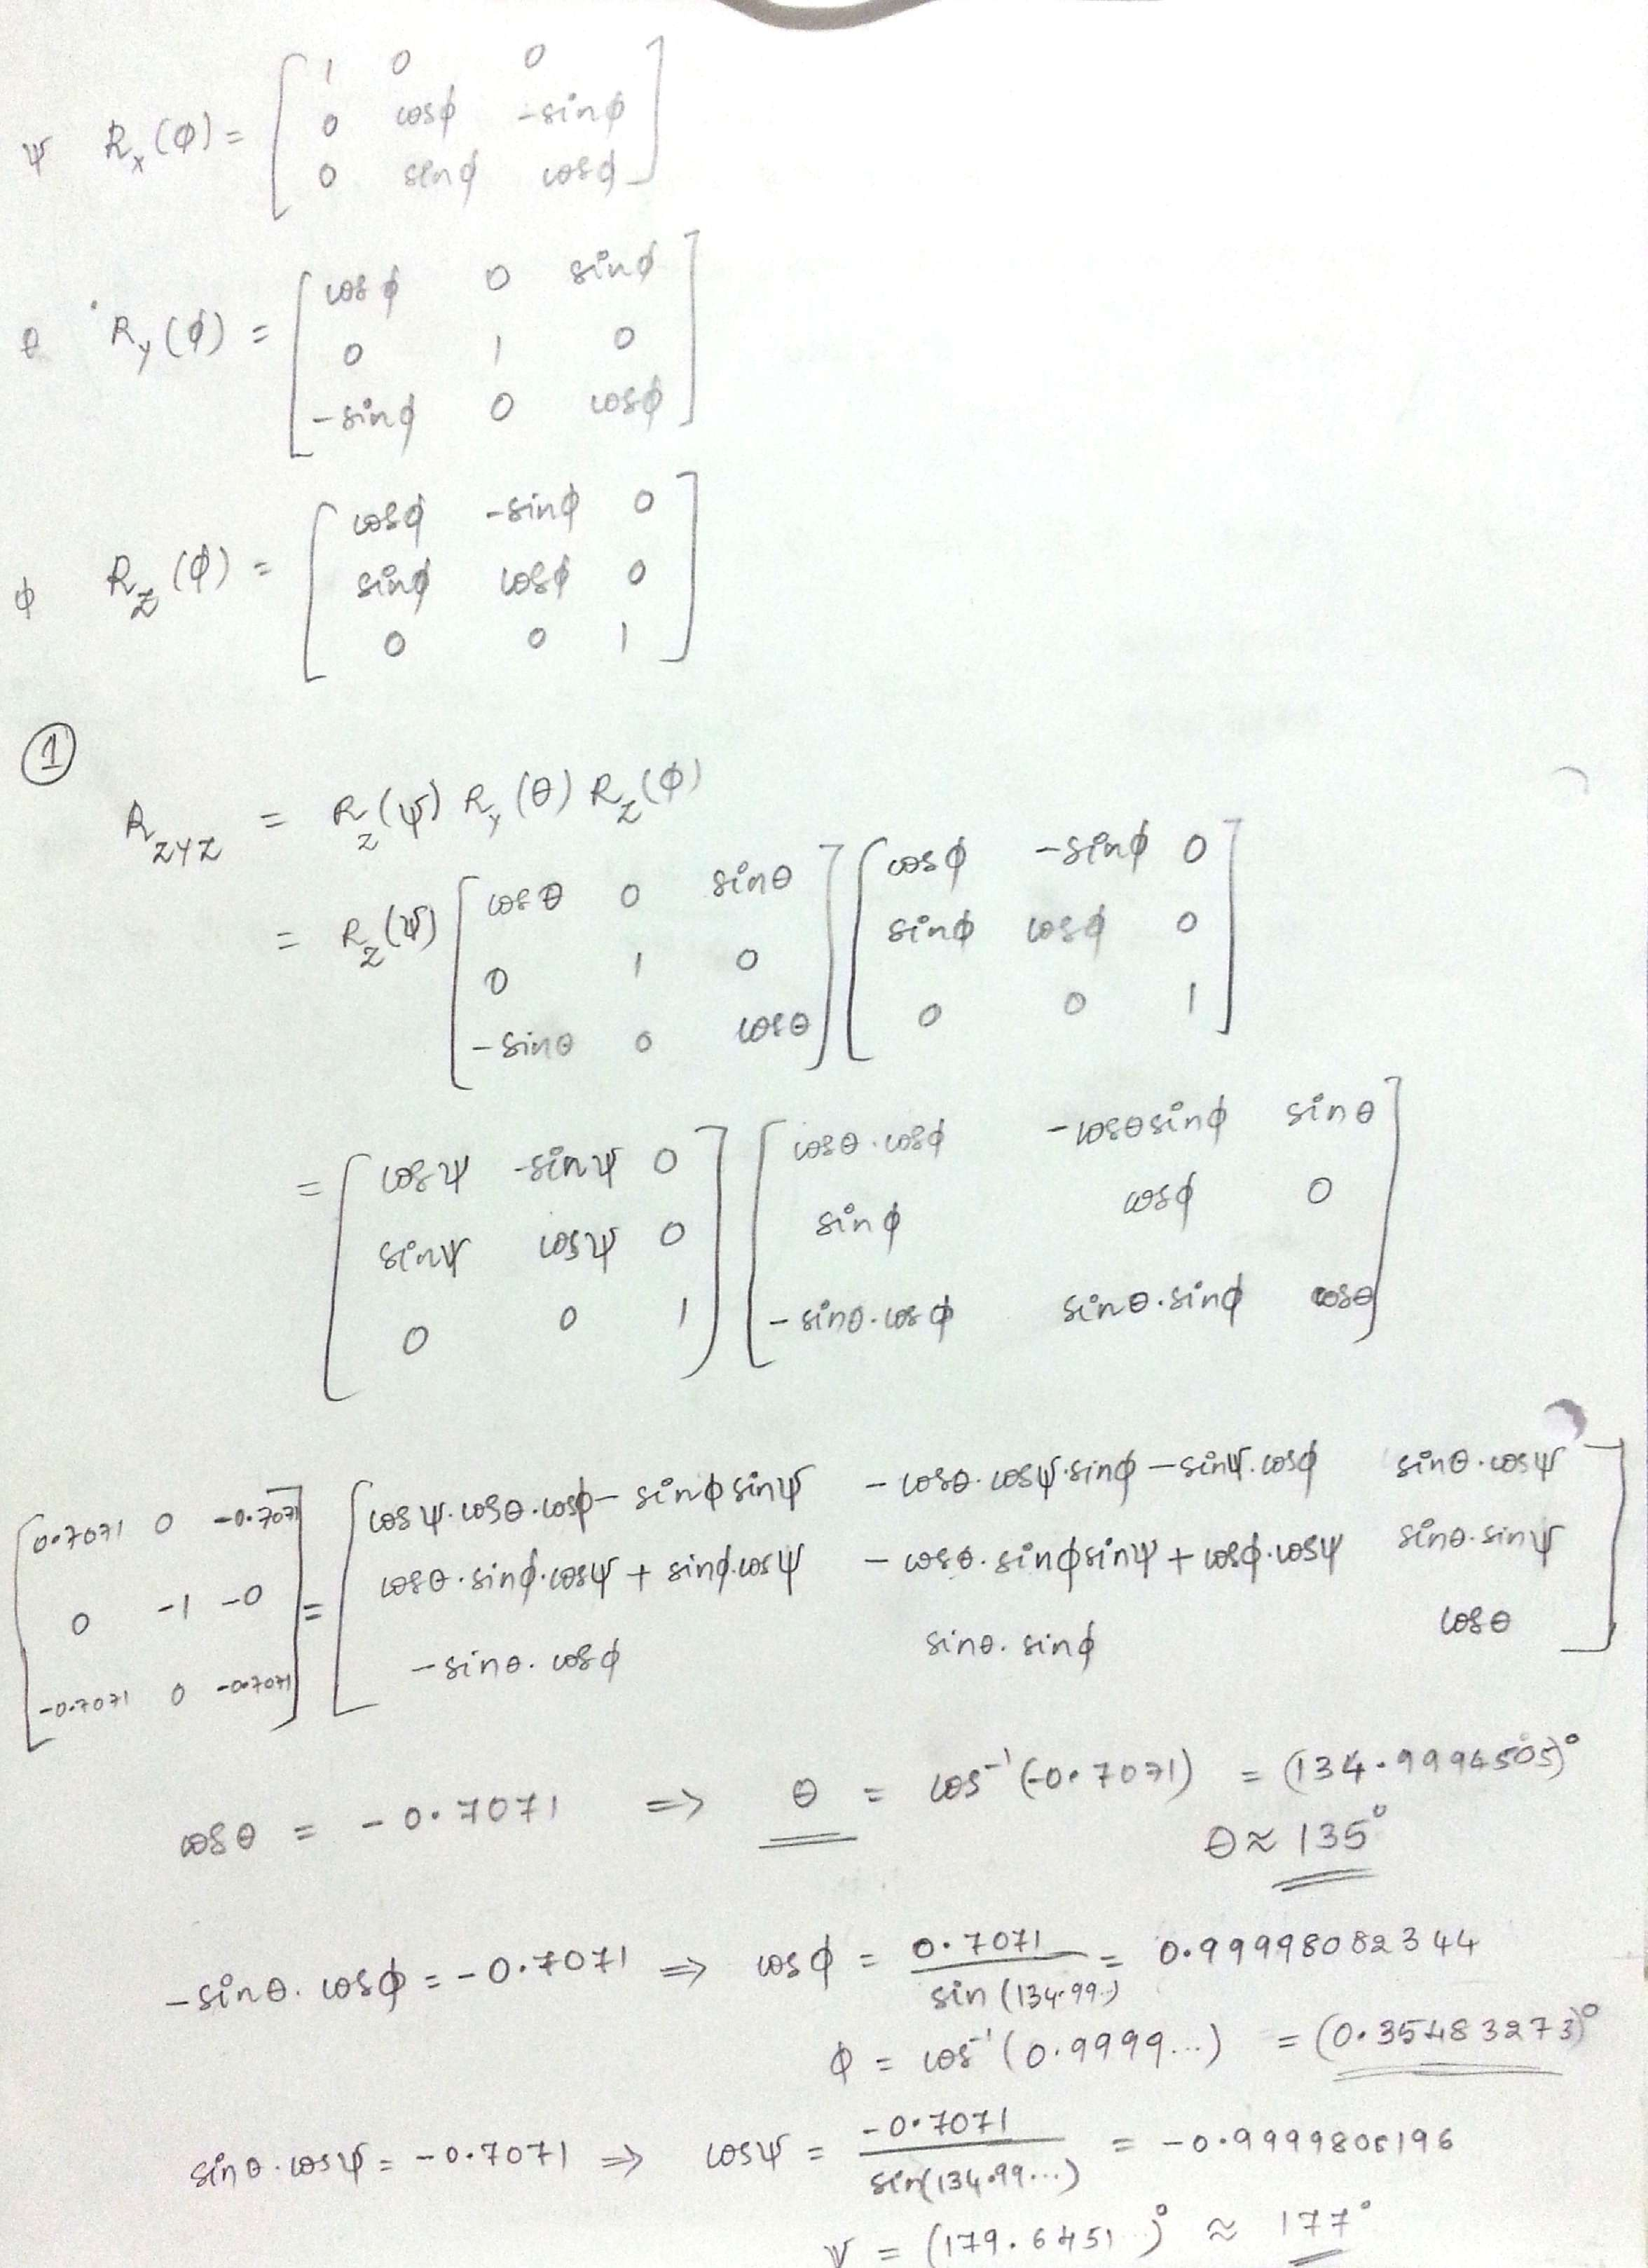
\includegraphics[width=\linewidth]{ex_05_1_1}\\
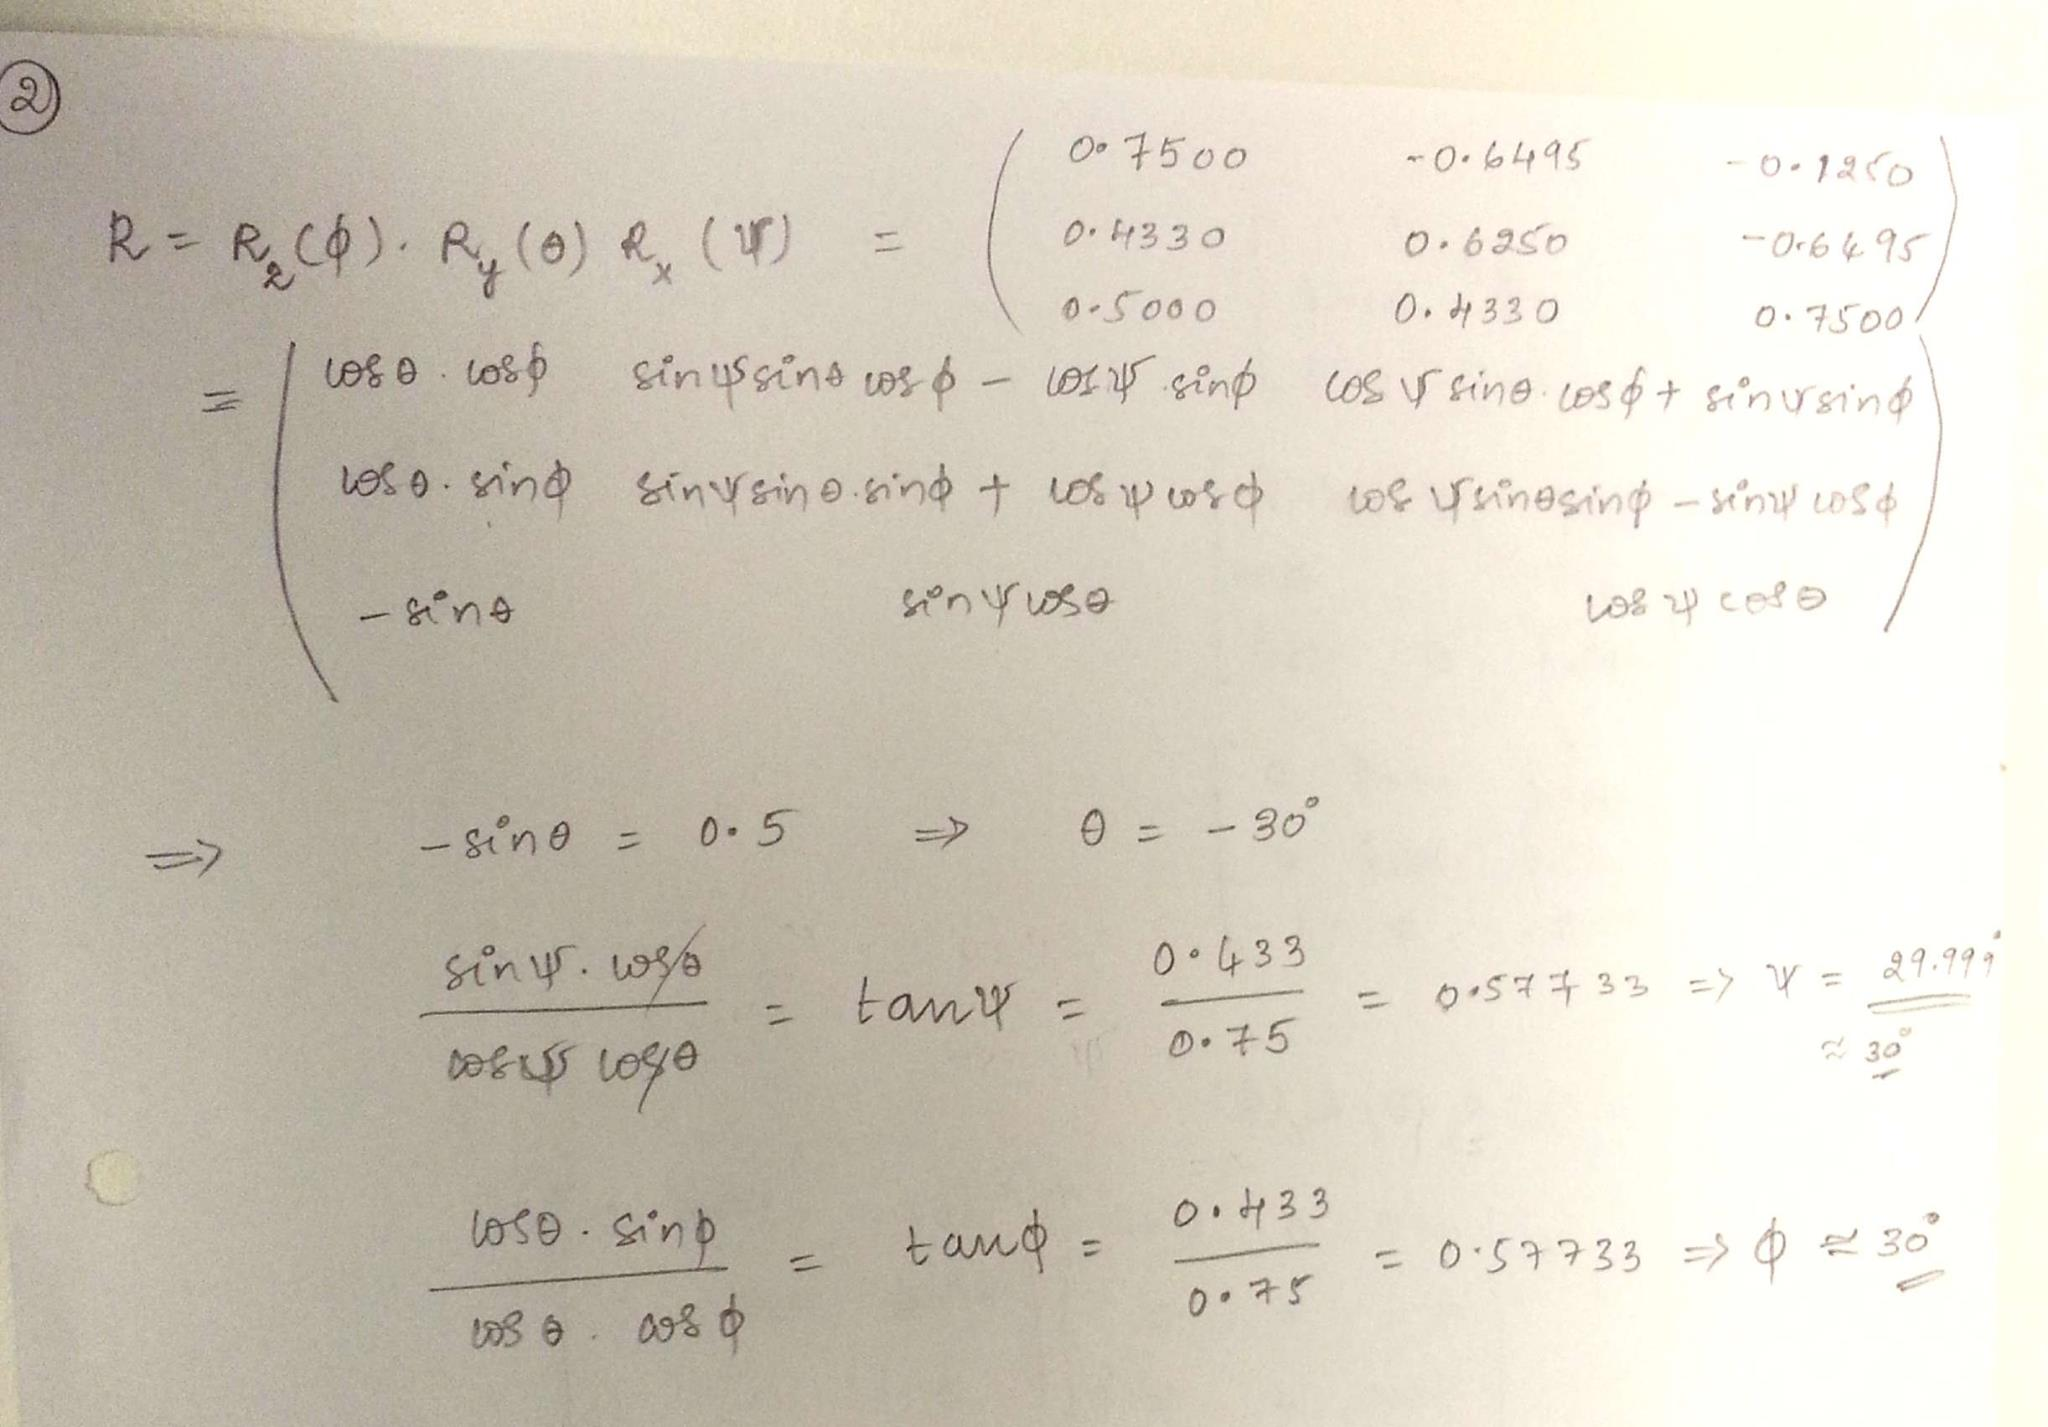
\includegraphics[width=\linewidth]{ex_05_1_2}\\

\subsection*{5.1-1}
\begin{itemize}
	\item pushMatrix
	\begin{itemize}
	\item Translate $V_i$ by $-V_1$, such that $V_1$ is at coordinate center.
	\item Rotate $V_i$ by 45$^{\circ}$
	\end{itemize}
	\item popMatrix()
	\item Translate $V_i$ by $+V_1$ (old)
\end{itemize}


\subsection*{5.1-2} The sun is in the coordinate center, rotates around itself (y axis) with arbitrary angle $\phi_{sun}$, earth rotates around the original y axis (not the rotating one) around coordinate center with angle  $\frac{360}{365}^{\circ}$, then there has to be a rotation about the new, by 23.5$^{\circ}$ rotated, y-axis by $\phi_{earth}$, the moon rotates around the translated and rotating y-axis (but in x-z-layer, not the rotated axes).
\begin{itemize}
\item Set $sun$, $earth$ and $moon$ to coordinate center.
\item PushMatrix()
\begin{itemize}
\item Rotate $sun$ about angle $\phi_{sun}$ around y-axis
\end{itemize}
\item popMatrix()
\end{itemize}


\begin{itemize}
\item PushMatrix()
\begin{itemize}
\item Rotate $earth$ about $\frac{360}{365}^{\circ}$ around y-axis
\item Translate $earth$ and $moon$ about $dist_{earth-sun}$
\item PushMatrix()
\begin{itemize}
\item Rotate $earth$ about $23.5^{\circ}$ around z-axis
\item Rotate $earth$ about $\phi_{earth}$ around y-axis
\end{itemize}
\item PopMatrix()
\item PushMatrix()
\begin{itemize}
\item Rotate $moon$ about $\frac{360}{12}^{\circ}$ around y-axis
\item Translate $moon$ about $dist_{moon-earth}$
\end{itemize}
\item PopMatrix()
\end{itemize}

\item popMatrix()
\end{itemize}
\end{document}